\documentclass[aspectratio=169]{beamer}
\usetheme{Madrid}
\usefonttheme{structurebold}
\usefonttheme[onlymath]{serif}

\definecolor{BKTemplate}{rgb}{0.11765, 0.30588, 0.47451}
\usecolortheme[named=BKTemplate]{structure}
\setbeamercolor{title}{fg=BKTemplate,bg=}
\setbeamertemplate{caption}[default]
\setbeamertemplate{navigation symbols}{}

\setbeamertemplate{footline}{%
  \hfill%
  \usebeamerfont{page number in head/foot}%
  \insertframenumber\,/\,\inserttotalframenumber%
  \hspace{1.5ex}\vspace{1ex}%
}

\usepackage{url}
\usepackage{booktabs}
\usepackage{amsfonts}
\usepackage{microtype}
\usepackage{multicol}
\usepackage{xcolor}
\usepackage{colortbl}
\usepackage{graphicx}
\usepackage{tikz}
\usetikzlibrary{positioning, arrows.meta}
\usepackage{amsmath}
\usepackage{tabularx}

\graphicspath{{images/}{../image/}}

\renewcommand{\footnotesize}{\tiny}

%------------------------------------------------------------
\title[Streaming Lakehouse Data Platform]
{\vspace*{0.5cm}\\\textbf{VIETTEL DIGITAL TALENT 2026}\\\textbf{Streaming Lakehouse Data Platform}}

\subtitle{Learning how a modern streaming platform works, end to end}

\author[Ngo Quang Hieu]{
  Mentor: Nguyen Minh Hieu \\
  Student: Ngo Quang Hieu
}

\institute[VDT 2026]{
  Data Engineer Track \\
  Viettel Digital Talent 2026
}

\date[July 2026]{July 1$^{st}$, 2026}
%------------------------------------------------------------

\begin{document}

% ── Title ─────────────────────────────────────────────────────────────────────
\setbeamertemplate{background canvas}{
  
\includegraphics[width=\paperwidth,height=\paperheight]{images/FrontBackgroundvtt.png}
}
\begin{frame}[plain]
\titlepage
\end{frame}

\setbeamertemplate{background canvas}{
  
\includegraphics[width=\paperwidth,height=\paperheight]{images/Backgroundvtt.png}
}

\begin{frame}{Table of Contents}
\tableofcontents
\end{frame}

%=============================================================================
\section{Introduction}
%=============================================================================

\begin{frame}{Motivation \& Goals}
\begin{columns}
  \column{0.5\textwidth}
  \textbf{Why a streaming lakehouse}
  \begin{itemize}\small
    \item A music-streaming platform produces a continuous stream of small events, not daily batches
    \item Batch ETL is always some interval behind reality -- fine for reports, too slow for "what is happening now"
    \item Doing this reliably (not just fast) means solving ordering, fault tolerance, exactly-once delivery, and read/write contention
  \end{itemize}

  \column{0.47\textwidth}
  \textbf{Goals}
  \begin{itemize}\small
    \item Build a working, end-to-end streaming lakehouse pipeline and learn how a modern streaming platform works
    \item Apply distributed-systems concepts from the course to a real system: partitioning, replication, exactly-once processing, lag monitoring
    \item Make the whole system observable and reproducible -- single Docker Compose command
  \end{itemize}
\end{columns}
\end{frame}

%=============================================================================
\section{Background \& Theory}
%=============================================================================

\begin{frame}{Core Concepts}
\begin{columns}
  \column{0.48\textwidth}
  \textbf{Message queue (pub-sub)}
  \begin{itemize}\small
    \item Producers append to a durable, ordered log; consumers subscribe independently, at their own pace
    \item Decouples producers from consumers in both time and number
  \end{itemize}
  \vspace{0.15cm}
  \textbf{Batch vs.\ streaming engine}
  \begin{itemize}\small
    \item Batch: bounded input, runs once, stops
    \item Streaming: unbounded input, engine never stops waiting for the next event (micro-batch or event-at-a-time)
  \end{itemize}

  \column{0.48\textwidth}
  \textbf{Storage \& open table formats}
  \begin{itemize}\small
    \item Lakehouse = object storage (cheap, scalable) + an open table format on top for ACID upserts and time travel
    \item COPY\_ON\_WRITE -- fast reads, expensive writes; MERGE\_ON\_READ -- cheap streaming appends, merged at read time
  \end{itemize}
  \vspace{0.15cm}
  \textbf{Medallion layering}
  \begin{itemize}\small
    \item Bronze (raw) $\to$ silver (cleaned) $\to$ gold (modeled)
    \item This project: bronze $\to$ gold directly -- dataset is small and clean enough to skip silver
  \end{itemize}
\end{columns}
\end{frame}

%=============================================================================
\section{Problem \& Challenges}
%=============================================================================

\begin{frame}{The Problem Before Streaming Lakehouses}
  \begin{itemize}\setlength\itemsep{5pt}
    \item \textbf{Batch ETL latency} -- dashboards always reflect the last scheduled load, not the current state
    \item \textbf{Lambda-architecture complexity} -- a batch layer and a separate real-time speed layer duplicate the same logic in two codebases
    \item \textbf{No serving layer on the lake} -- plain object storage has no row-level update/delete or ACID transactions; the lake stayed a read-only dump
    \item \textbf{Storage and compute coupled} -- traditional warehouses force paying for both together, so teams kept two copies of the same data
  \end{itemize}
  \vspace{0.2cm}
  \textbf{This project's concrete challenges:} keeping up with Eventsim's continuous arrival rate across 3 Kafka topics, exactly-once fault-tolerant processing on a 2-node cluster, and fitting everything inside a fixed, shared 4-core Spark budget.
\end{frame}

%=============================================================================
\section{Proposed Solution}
%=============================================================================

\begin{frame}{Streamify: End-to-End Architecture}
\centering

\includegraphics[width=0.82\textwidth]{app/overview.png}
\end{frame}

\begin{frame}{Ingestion Layer: Apache Kafka}
\begin{columns}
  \column{0.52\textwidth}
  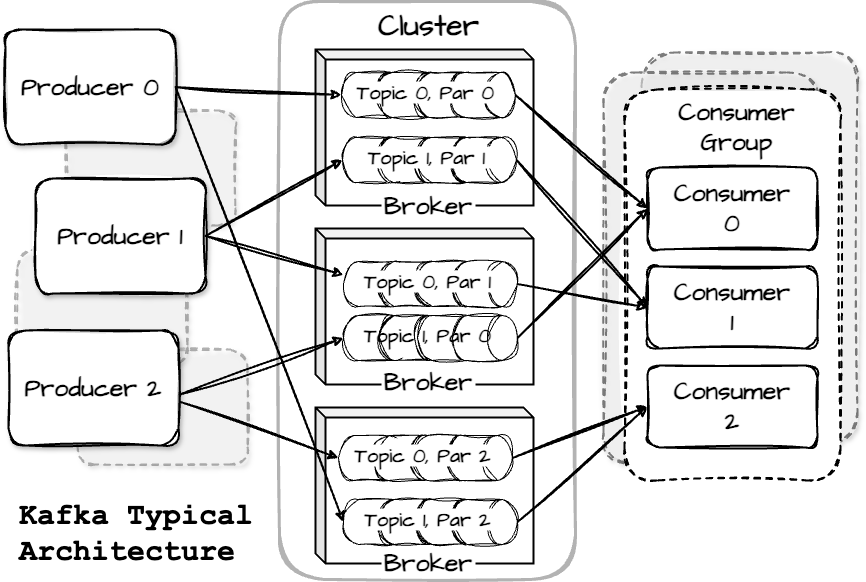
\includegraphics[width=\textwidth]{kafka/kafka_architecture.png}

  \column{0.45\textwidth}
  \begin{itemize}\small
    \item 2-node KRaft cluster (\texttt{broker-1}, \texttt{broker-2}) -- no ZooKeeper, each node is broker \& controller
    \item 3 topics (\texttt{listen\_events}, \texttt{page\_view\_events}, \texttt{auth\_events}), 3 partitions each, replication factor 2
    \item Every partition has a leader on one broker and a follower on the other -- follower takes over if its broker fails
  \end{itemize}
\end{columns}
\end{frame}

\begin{frame}{Stream Processing: Spark Structured Streaming $\to$ Hudi Bronze}
\begin{columns}
  \column{0.55\textwidth}
  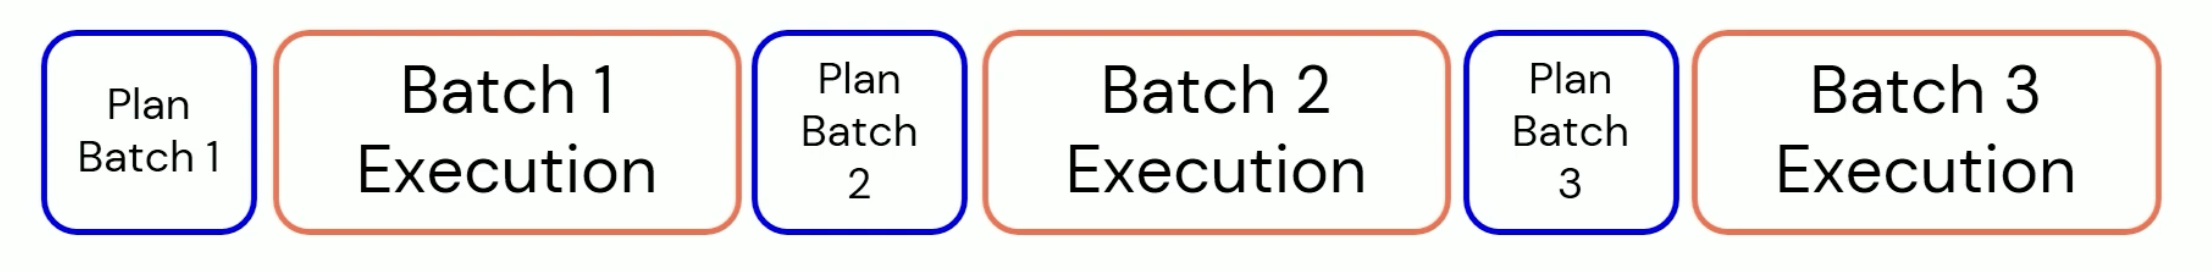
\includegraphics[width=\textwidth]{engine/spark_micro_batch.png}
  \par\vspace{2pt}{\tiny Driver polls Kafka, groups new records into a micro-batch, runs it as a Spark job}

  \column{0.42\textwidth}
  \begin{itemize}\small
    \item Reads all 3 topics, fixes latin1-mojibake, derives time columns, appends to \texttt{staging.<topic>} (Hudi MERGE\_ON\_READ)
    \item Checkpoint volume tracks Kafka offsets and query state -- resumes exactly where it left off on restart
    \item Shares the 4-core Spark Standalone cluster with the dbt Thrift Server, 2 cores each
  \end{itemize}
\end{columns}
\end{frame}

\begin{frame}{Transformation \& Serving}
\begin{columns}
  \column{0.5\textwidth}
  \centering
  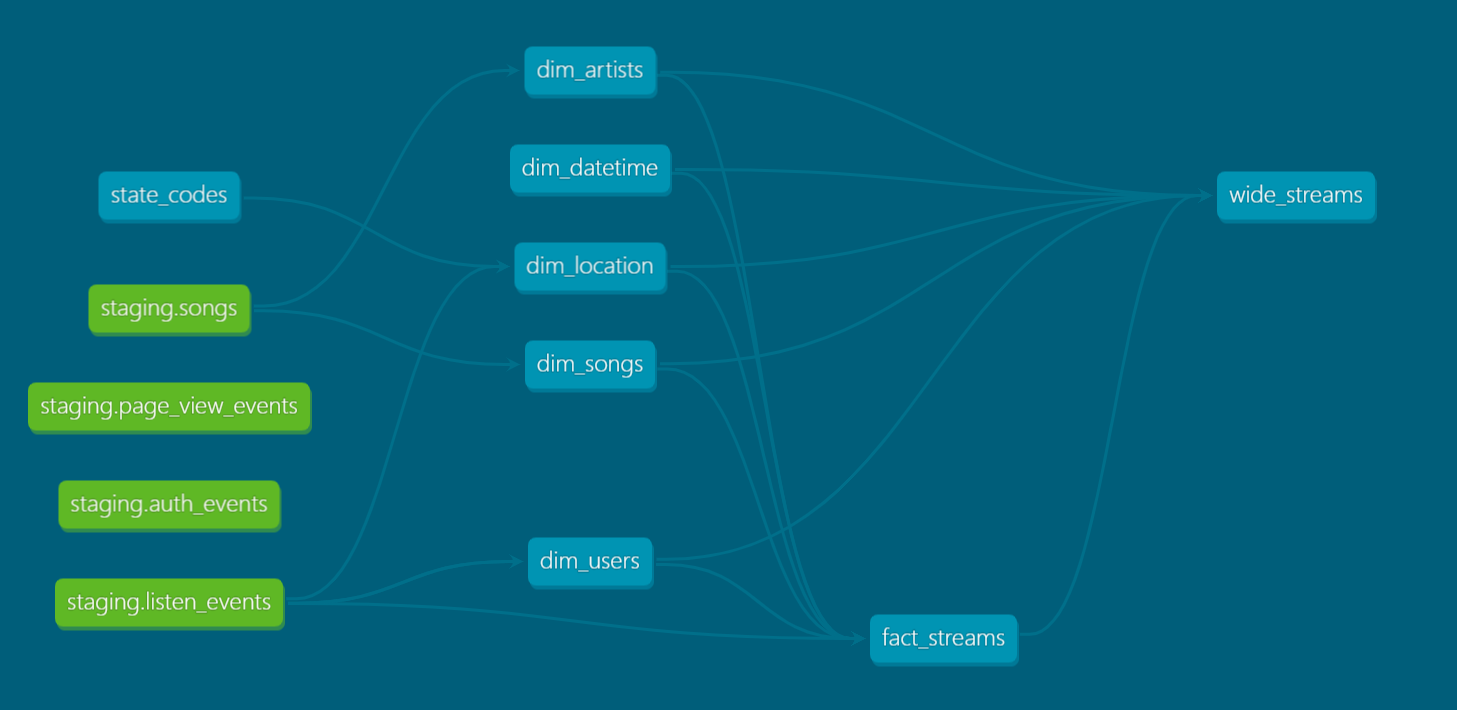
\includegraphics[width=\textwidth]{app/dbt_graph.png}
  \column{0.48\textwidth}
  \begin{itemize}\small
    \item dbt builds a \textbf{star schema} (\texttt{fact\_streams} + 5 dims) and a denormalized \textbf{wide\_streams} table straight from bronze, via the Spark Thrift Server
    \item Both materialized as COPY\_ON\_WRITE Hudi tables, rebuilt each run
    \item \textbf{Superset} queries \texttt{wide\_streams} through the same Thrift Server -- one flat table, no dashboard-time joins
  \end{itemize}
\end{columns}
\vspace{0.2cm}
\centering

\includegraphics[width=0.55\textwidth]{app/dashboard.png}
\end{frame}

\begin{frame}{Monitoring Layer}
\begin{columns}
  \column{0.48\textwidth}
  \begin{itemize}\small
    \item \textbf{kafka-exporter} -- per-partition consumer-group lag
    \item \textbf{Spark's Prometheus endpoint} -- job/JVM metrics
    \item \textbf{cAdvisor} -- per-container CPU/memory
    \item Grafana renders lag and Spark job health so the system's health is visible, not just whether it is running
  \end{itemize}
  \column{0.48\textwidth}
  \centering
  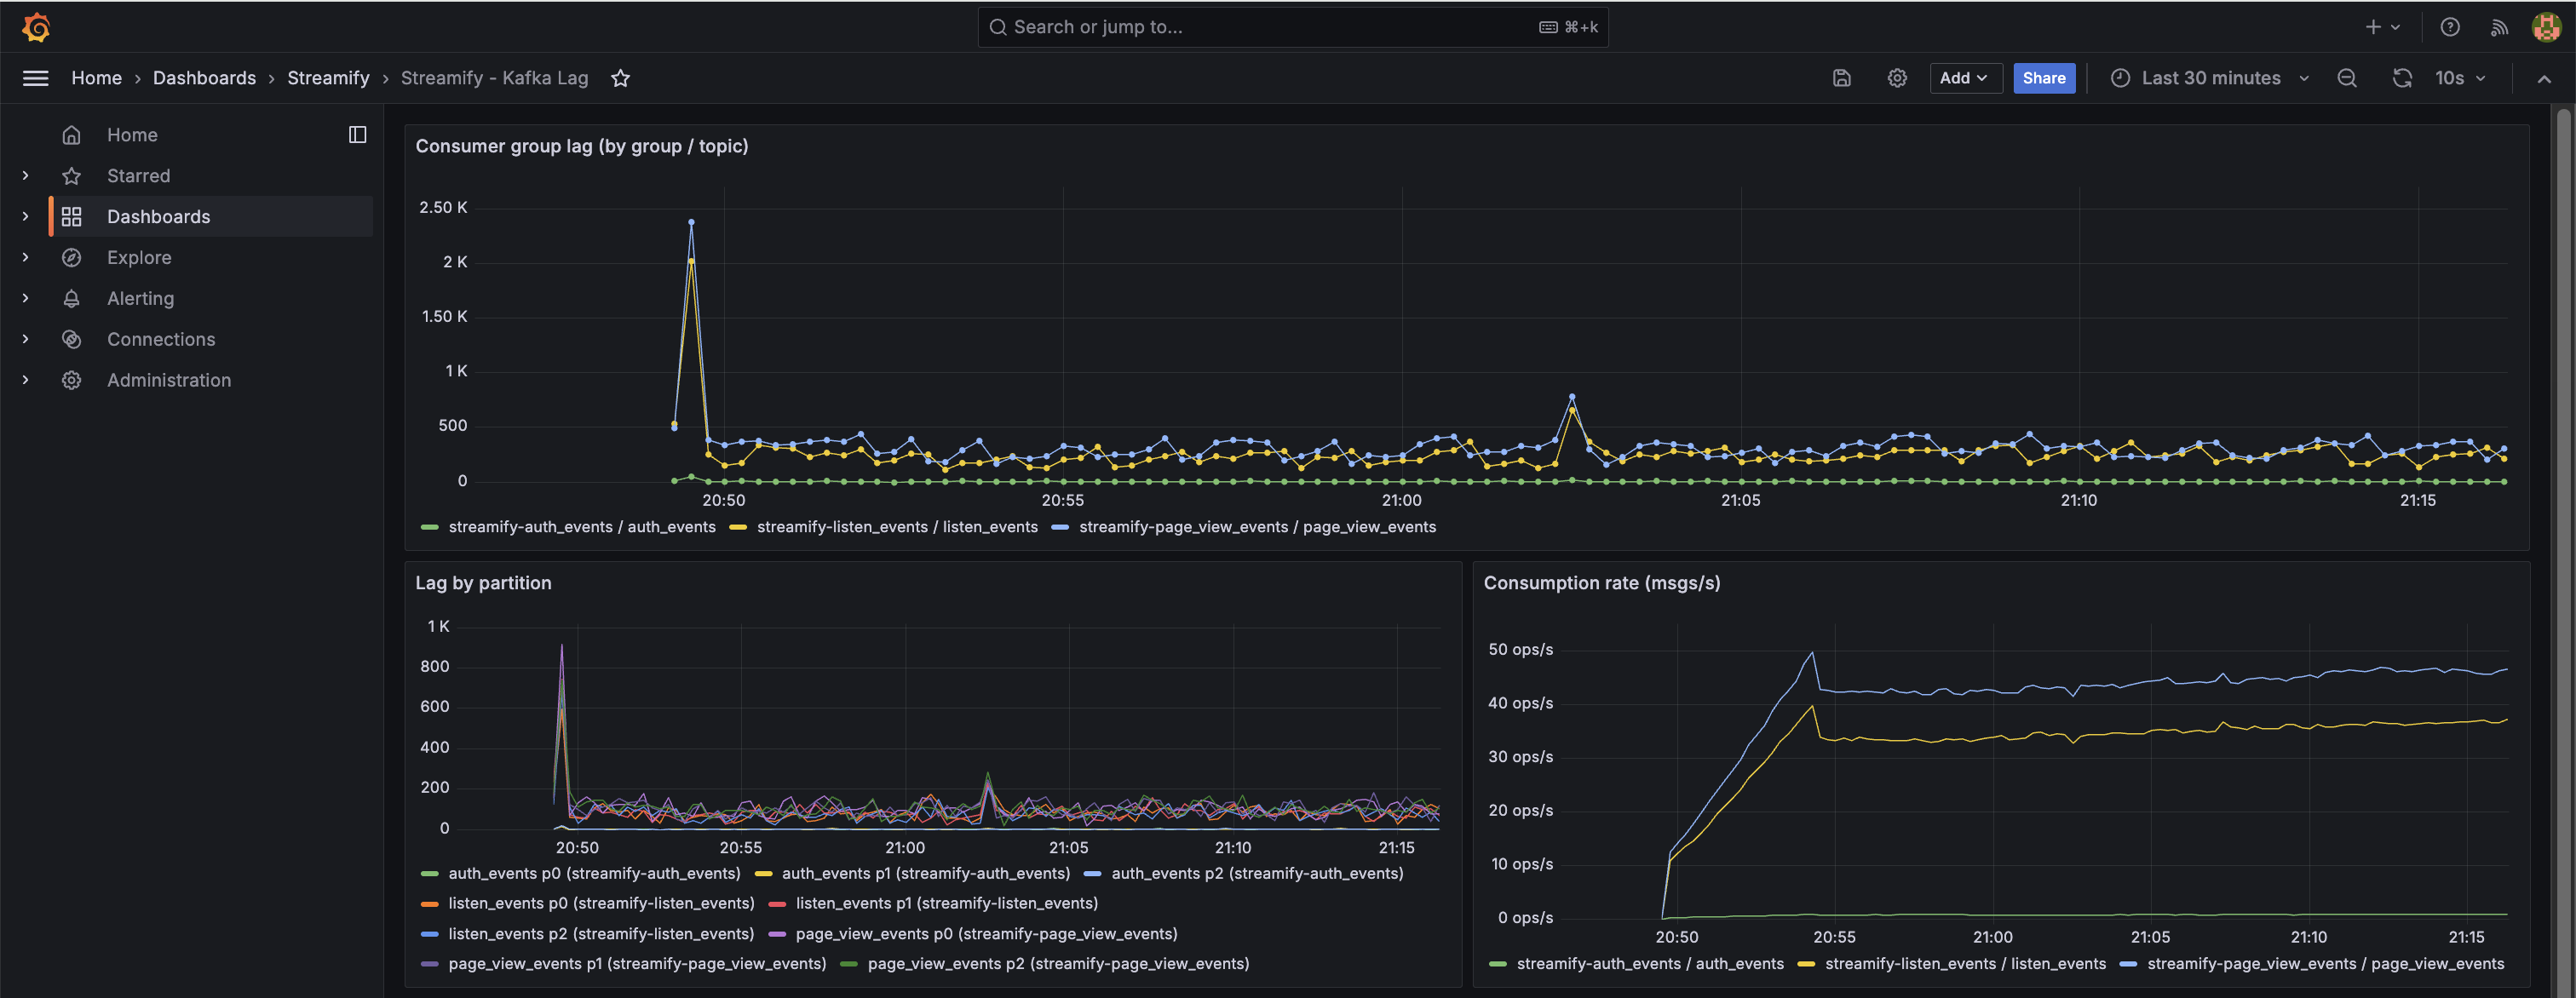
\includegraphics[width=\textwidth]{grafana_kafka.png}
\end{columns}
\end{frame}

%=============================================================================
\section{Conclusion}
%=============================================================================

\begin{frame}{Conclusion}
\textbf{Results Achieved}
\begin{itemize}\setlength\itemsep{4pt}\small
  \item Understood, hands-on, how a streaming platform works end to end: why a Kafka partition needs a follower replica, why the Structured Streaming checkpoint is separate from the consumer-group offset, when MERGE\_ON\_READ is worth its read-time cost
  \item Exercised partitioning, replication, checkpointed exactly-once processing, and lag observability against real failure modes, not just in theory
  \item Confirmed why the streaming-lakehouse pattern closes the batch/lambda-architecture gaps: no duplicated speed-layer logic, a transactionally-updatable lake, storage and compute that scale independently
\end{itemize}

\vspace{0.2cm}
\textbf{Limitations}
\begin{itemize}\small
  \item Small, fixed 4-core Spark cluster, no autoscaling
  \item Synthetic Eventsim dataset, not validated against real production traffic
\end{itemize}

\vspace{0.2cm}
\textbf{Future Directions}
\begin{itemize}\small
  \item Real or real-scale streaming dataset; autoscaled Kafka/Spark cluster
  \item Alerting on consumer lag and job failures; a silver layer once bronze needs cleaning
\end{itemize}
\end{frame}

%=============================================================================
\section{References}
%=============================================================================

\begin{frame}{References}
  \begin{itemize}\small
    \item Apache Kafka Documentation. \url{https://kafka.apache.org/documentation/}
    \item Spark Structured Streaming Programming Guide. \url{https://spark.apache.org/docs/latest/structured-streaming-programming-guide.html}
    \item Apache Hudi Documentation. \url{https://hudi.apache.org/docs/overview}
    \item dbt Documentation (dbt-spark adapter). \url{https://docs.getdbt.com/docs/core/connect-data-platform/spark-setup}
    \item Apache Superset Documentation. \url{https://superset.apache.org/docs/intro}
    \item Eventsim (viirya's fork). \url{https://github.com/viirya/eventsim}
    \item Million Song Dataset. \url{http://millionsongdataset.com}
  \end{itemize}
\end{frame}

% ── The End ───────────────────────────────────────────────────────────────────
\setbeamertemplate{footline}{}
\begin{frame}
  \centering
  \vspace{1.2cm}
  \textbf{\Huge{- THE END -}}\\
  \vspace{0.5cm}
  \textit{\Large{Thank you for your attention}}\\
  \vspace{0.5cm}
  \textbf{Contact:}\\
  Ngo Quang Hieu --- Viettel Digital Talent 2026
\end{frame}

\end{document}
